\chapter{Scale setting}%\addcontentsline{toc}{chapter}{Scale setting}

%%%%%%%%%%%%%%%%%%%%%%%%%%%%%%%%%%%%%%%%%%%%%%%%%%%%%%%%%%%
%%%%%%%%%%%%%%%%%%%%%%%%%%%%%%%%%%%%%%%%%%%%%%%%%%%%%%%%%%%
%%%%%%%%%%%%%%%%%%%%%%%%%%%%%%%%%%%%%%%%%%%%%%%%%%%%%%%%%%%
%%%%%%%%%%%%%%%%%%%%%%%%%%%%%%%%%%%%%%%%%%%%%%%%%%%%%%%%%%%

\label{ch_ss}

%%%%%%%%%%%%%%%%%%%%%%%%%%%%%%%%%%%%%%%%%%%%%%%%%%%%%%%%%%%
%%%%%%%%%%%%%%%%%%%%%%%%%%%%%%%%%%%%%%%%%%%%%%%%%%%%%%%%%%%
%%%%%%%%%%%%%%%%%%%%%%%%%%%%%%%%%%%%%%%%%%%%%%%%%%%%%%%%%%%
%%%%%%%%%%%%%%%%%%%%%%%%%%%%%%%%%%%%%%%%%%%%%%%%%%%%%%%%%%%

\section{Motivation}
\label{ch_ss:sec:introduction}

The scale setting involves the precise determination of one reference observable, the scale, in physical units, to which any other observable is compared in order to extract the value of the latter in physical units. 

We decide to use the gradient flow scale $t_0$ introduced in Sec.~\ref{ch_observables:sec:Flow} as an intermediate reference scale since it can be computed in the lattice with high precision. Following the discussion in Sec.~\ref{ch_foundation:sec:ss}, we choose for the phenomenological input the linear combination of the decay constants of the pion and kaon
\begin{equation}
\label{ch_ss:eq:fpik}
\Lambda\equiv f_{\pi K}=\frac{2}{3}\left(f_K+\frac{1}{2}f_{\pi}\right).
\end{equation}
After measuring $\sqrt{t_0}f_{\pi K}$ for each ensemble, one must perform a chiral-continuum limit in order to extract its value at physical quark masses and in the continuum. To define the physical point we use the pion and kaon physical masses, or equivalently the dimensionless quantities $\phi_2$ and $\phi_4$. Thanks to the mass shifting procedure in Sec.~\ref{ch_ma:sec:chiral_traj}, the value of $\phi_4$ is fixed to its physical value along our trajectory in the quark mass plane, so the chiral extrapolation needs to be done in $\phi_2$ only. For the determination of the physical value of the latter we use the initial guess in eq.~(\ref{ch_ma:eq:t0_guess}) and the physical input in eq.~(\ref{ch_ss:eq:isoQCD}). As commented in Sec.~\ref{ch_ma:sec:chiral_traj}, once a new determination of $t_0$ at the physical point is obtained, the analysis is iterated updating the value in eq.~(\ref{ch_ma:eq:t0_guess}) until convergence is observed. Thus, with each iterative step both the values of $\phi_2$ to which we perform the chiral extrapolation and the value of $\phi_4$ to which we shift our observables are updated. 

Since all lattice observables and the action that we use are $\mathcal{O}(a)$ improved, we expect lattice artifacts to start at $\mathcal{O}(a^2)$ for $\sqrt{t_0}f_{\pi K}$.

In order to perform the chiral-continuum limit, we explore different ways of parameterizing the dependence on $\phi_2$ ($\phi_4$ is constant thanks to the mass shifting procedure of Sec.~\ref{ch_ma:sec:chiral_traj}) and on the lattice spacing $a$, and employ the same techniques of model averaging discussed in Sec.~\ref{ch_observables:sec:MA}.

After performing the chiral-continuum limit, using as external physical input the values of the pion and kaon decay constants we can determine the value of the scale $t_0$ as
\begin{equation}
\sqrt{t_0^{\textrm{ph}}}=\frac{\left.\left(\sqrt{t_0}f_{\pi K}\right)^{\textrm{latt}}\right|_
{\phi_2^{\textrm{ph}},\;a=0}}{f_{\pi K}^{\textrm{exp}}}.
\end{equation}

In particular, we are studying ensembles which employ $N_f=2+1$ fermions, and thus assume isospin symmetry for the up and down flavors. This means that the physical input for the masses and decay constants we need is not that of Nature, but that of isosymmetric QCD (isoQCD). These values are given by the Flavor Lattice Average Group (FLAG) in~\citep{FlavourLatticeAveragingGroupFLAG:2021npn}
\begin{gather}
\label{ch_ss:eq:isoQCD}
m_{\pi}^{\textrm{isoQCD}}=134.9768(5)\;{\textrm{MeV}}, \quad
m_{K}^{\textrm{isoQCD}}=497.611(13)\;{\textrm{MeV}}, \\
f_{\pi}^{\textrm{isoQCD}}=130.56(2)_{\textrm{exp}}(13)_{\textrm{QED}}(2)_{|V_{ud}|}\;{\textrm{MeV}}, \quad \\
f_{K}^{\textrm{isoQCD}}=157.2(2)_{\textrm{exp}}(2)_{\textrm{QED}}(4)_{|V_{us}|}\;{\textrm{MeV}}.
\end{gather} 
As we see, the kaon decay constant receives a large contribution to its uncertainty from the determination of the $|V_{us}|$ CKM matrix element. Also, QED corrections are stronger in the kaon than in the pion decay constant. All these subtleties motivate a scale setting that uses only the pion decay constant as physical input. For this reason we will also study this possibility when doing the model variation for the chiral-continuum extrapolation.

%%%%%%%%%%%%%%%%%%%%%%%%%%%%%%%%%%%%%%%%%%%%%%%%%%%%%%%%%%%
%%%%%%%%%%%%%%%%%%%%%%%%%%%%%%%%%%%%%%%%%%%%%%%%%%%%%%%%%%%
%%%%%%%%%%%%%%%%%%%%%%%%%%%%%%%%%%%%%%%%%%%%%%%%%%%%%%%%%%%
%%%%%%%%%%%%%%%%%%%%%%%%%%%%%%%%%%%%%%%%%%%%%%%%%%%%%%%%%%%


\section{Results: the physical point}
\label{ch_ss:sec:Results}

The choice of the combination of decay constants $f_{\pi K}$ in eq.~(\ref{ch_ss:eq:fpik}) to set the scale is due to its chiral behavior, since at fixed value of $\phi_4$ (as in our case thanks to the mass shifting procedure, see Sec.~\ref{ch_ma:sec:chiral_traj}) to NLO $SU(3)$ ChPT it only depends on $\phi_2$ through chiral logarithms. To this order we have, using $m_u=m_d\equiv m_l$~\citep{FLAG16,Bar:2013ora}
\begin{align}
t_0&=t_{0,\textrm{ch}}\left(1+k_1\frac{2m_K^2+m_{\pi}^2}{(4\pi f)^2}\right), \\
m_{\pi}^2&=2B_0m_l, \\
m_K^2&=B_0(m_l+m_s), \\
m_{\eta}^2&=\frac{4}{3}m_K^2-\frac{1}{3}m_{\pi}^2, \\
f_{\pi}&=f\left[1+\frac{16B_0L_5}{f^2}m_l+\frac{16B_0L_4}{f^2}(2m_l+m_s)-2L(m_{\pi}^2)\right. \\
&\left.-L(m_K^2)\right], \\
f_K&=f\left[1+\frac{8B_0L_5}{f^2}(m_l+m_s)+\frac{16B_0L_4}{f^2}(2m_l+m_s)\right. \\
&\left.-\frac{3}{4}L(m_{\pi}^2)-\frac{3}{2}L(m_K^2)-\frac{3}{4}L(m_{\eta}^2)\right],
\end{align}
where $L(x)$ are chiral logarithms, defined as
\begin{equation}
L(x)=\frac{x}{(4\pi f)^2}\textrm{log}\frac{x}{(4\pi f)^2},
\end{equation}
and $f,t_{0,\textrm{ch}},k_1,B_0,L_i$ are low energy constants (LECs). The combination $\sqrt{8t_0}f_{\pi K}$ reads
\begin{align}
\label{ch_ss:eq:SU3ChPT}
F_{\chi,\pi K}^{\textrm{cont}}(\phi_2)&\equiv\left(\sqrt{8t_0}f_{\pi K}\right)^{\textrm{cont}}=\\
&=\frac{A}{4\pi}\left[1-\frac{7}{6}\tilde{L}\left(\frac{\phi_2}{A^2}\right)-\frac{4}{3}\tilde{L}\left(\frac{\phi_4-\frac{1}{2}\phi_2}{A^2}\right)\right. \\
&\left.-\frac{1}{2}\tilde{L}\left(\frac{\frac{4}{3}\phi_4-\phi_2}{A^2}\right)+\frac{B}{A^2}\phi_4\right],
\end{align}
with modified chiral logarithms given by
\begin{equation}
\label{ch_ss:eq:log}
\tilde{L}(x)=x{\textrm{log}}\left(x\right),
\end{equation}
and where we absorbed the LECs into the definition of the parameters $A,B$ as
\begin{align}
A&=4\pi\sqrt{8t_{0,\textrm{ch}}}f, \\
B&=\frac{(16\pi)^2}{3}(L_5+3L_4)+k_1.
\end{align} 
We use the expression in eq.~(\ref{ch_ss:eq:SU3ChPT}) to perform the chiral-continuum extrapolation of $\sqrt{8t_0}f_{\pi K}$. We will use the label $[SU(3)\chi PT]$ for this continuum dependence. 

Another possibility for the physical point extrapolation is to use Taylor expansions in $\phi_2$ around the symmetric point. We can either go to second or fourth order in the Taylor expansion
\begin{equation}
\label{ch_ss:eq:Tay}
F_{\textrm{Tay},\pi K}^{\textrm{cont}}(\phi_2)\equiv\sqrt{8t_0}f_{\pi K}^{\textrm{cont}}=A+B\left(\phi_2-\phi_2^{\textrm{sym}}\right)^2,
\end{equation}
or
\begin{equation}
\label{ch_ss:eq:Tay4}
F_{\textrm{Tay},\pi K}^{\textrm{cont}}(\phi_2)=A+B\left(\phi_2-\phi_2^{\textrm{sym}}\right)^2+C\left(\phi_2-\phi_2^{\textrm{sym}}\right)^4,
\end{equation}
labeling these models as $[Tay]$ and $[Tay4]$. Due to symmetry reasons~\citep{Bietenholz:2011qq}, there are no terms with odd powers of $\phi_2-\phi_2^{\textrm{sym}}$.

In addition to the extrapolation in the pion mass, we need to supplement these fit functions with cutoff effects in order to describe our lattice data. For this we will explore three possibilities
\begin{align}
\label{ch_ss:eq:a2}
F^{\textrm{latt}}(\phi_2)&=F^{\textrm{cont}}(\phi_2)+W\frac{a^2}{8t_0},\\
\label{ch_ss:eq:aas}
F^{\textrm{latt}}(\phi_2)&=F^{\textrm{cont}}(\phi_2)+W\frac{a^2}{8t_0}\alpha_S^{\Gamma}(a),\\
\label{ch_ss:eq:a2phi2}
F^{\textrm{latt}}(\phi_2)&=F^{\textrm{cont}}(\phi_2)+\left(W+Z\phi_2\right)\frac{a^2}{8t_0}.
\end{align}
We assign the labels $[a^2]$, $[a^2\alpha_S^{\Gamma}]$ and $[a^2+a^2\phi_2]$ to characterize the lattice artifacts of these models. The lattce artifact in eq.~(\ref{ch_ss:eq:aas}) is motivated by~\citep{Husung:2022kvi} where logarithmic corrections in the lattice spacing $a$ where found to affect the continuum limit. In particular, a whole set of powers $\Gamma_i$ are found to contribute. However, due to the limited number of ensembles studied, sensitivity in this dependence is poor and we can only include one of these powers. We tested the impact of which value of $\Gamma_i$ to use and no change in the result for $t_0^{\textrm{ph}}$ was found for these models. Furthermore, all choices had the same value for the TIC in eq.~(\ref{ch_observables:eq:TIC}). For these reasons we choose to include in the final model average only the choice $\left(\Gamma_i\right)_{\textrm{min}}=-0.111$. For an estimation of $\alpha_S(a)$ we use
\begin{gather}
\alpha_S(a)\propto-\frac{1}{\textrm{log}\left(a\Lambda_{\overline{\textrm{MS}}}\right)}, \quad \Lambda_{\overline{\textrm{MS}}}^{(3)}=339(12)\;\textrm{MeV}~\citep{FlavourLatticeAveragingGroupFLAG:2021npn}.
\end{gather}

The systematic uncertainty in the extraction of $\sqrt{t_0^{\textrm{ph}}}$ is assessed by the model variation using the TIC introduced in Sec.~\ref{ch_observables:sec:MA}. We vary over the different ways of performing the chiral-continuum limits introduced above, as well as over the possibility of performing data cuts. In particular, we consider the following cuts (in addition to the ``no cut'' choice)
\begin{gather}
\beta>3.40, \quad
\beta>3.46, \quad
\phi_2<0.6, \\
\phi_2<0.4, \quad
\beta>3.40\;\&\;\phi_2<0.6, \\
m_{\pi}L>4.1.
\end{gather}

Finally, to perform all of these fits, we have two data sets: the Wilson unitary setup and the mixed action. Both must share the same continuum limit, but different cutoff effects. We can thus perform the continuum-chiral extrapolations for the Wilson data, for the mixed action, or for a combined data set, parameterizing the data with the same continuum limit behavior $F^{\textrm{cont}}(\phi_2)$ but different cutoff effects (different $W,Z$ fit parameters for Wilson and mixed action data). This third choice allows to further constrain the continuum extrapolation and keep it well under control, while increasing the statistics and getting better precision for $\sqrt{t_0^{\textrm{ph}}}$. As a universality check, we performed the continuum limit only of symmetric point ensembles of both the Wilson and mixed action data, without imposing a common value in the continuum. Since all these points have the same $\phi_2$ they follow a line of constant physics as we approach the continuum. This extrapolation is shown in Fig.~\ref{ch_ss:fig:universality} and indeed it shows that both data sets agree perfectly well in the continuum, with the mixed action data having much milder cutoff effects.

Once the various models to extrapolate to the continuum and physical point have been explored, we use the model averaging technique in Sec.~\ref{ch_observables:sec:MA} to assign a weight to each model 
\begin{equation}
\label{ch_ss:eq:W}
W\propto\exp\left(-\frac{1}{2}\left(\chi^2-2\left<\chi^2\right>\right)\right),
\end{equation}
that allows us to compute a weighted average for $\sqrt{t_0^{\textrm{ph}}}$, as well as the associated systematic uncertainty
\begin{align}
\left<\sqrt{t_0^{\textrm{ph}}}\right>&=\sum_i\sqrt{t_0^{\textrm{ph,}(i)}}W^{(i)},\\
\sigma^2_{\textrm{syst}}&=\left<\sqrt{t_0^2^{\textrm{,ph}}}\right>-\left<\sqrt{t_0^{\textrm{ph}}}\right>^2.
\end{align}

In Figs.~\ref{ch_ss:fig:BMA_w}-\ref{ch_ss:fig:BMA_comb} we show the model average results for the Wilson unitary setup, for the mixed action and for the combined analysis. In Appendix~\ref{apex_model_av_t0} we show the numerical results of $\sqrt{t_0^{\textrm{ph}}}$ for each model considered, together with their weights and p-values, for the Wilson, mixed action and combined analysis. In Fig.~\ref{ch_ss:fig:SU3a2} we show the pion mass dependence of the continuum-chiral extrapolation for model $[SU(3)\chi PT][a^2]$ and the combined data set (no cuts), together with the lattice spacing dependence for the same model, projecting all points to the physical pion mass $\phi_2^{\textrm{ph}}$ using the fit result for the continuum dependence $F^{\textrm{cont}}(\phi_2)$.

The final results for $\sqrt{t_0^{\textrm{ph}}}$ in physical units as computed from the model average for the different data sets, using $f_{\pi K}^{\textrm{isoQCD}}$ as physical input, are
\begin{align}
\label{ch_ss:eq:t0ph_w}
\sqrt{t_0^{\textrm{ph}}}&=0.1436(7)_{\textrm{stat}}(3)_{\textrm{syst}}\;\textrm{fm, Wilson}\;[f_{\pi K}], \\
\label{ch_ss:eq:t0ph_tm}
\sqrt{t_0^{\textrm{ph}}}&=0.1441(9)_{\textrm{stat}}(6)_{\textrm{syst}}\;\textrm{fm, Mixed action}\;[f_{\pi K}], \\
\label{ch_ss:eq:t0ph_c}
\sqrt{t_0^{\textrm{ph}}}&=0.1440(6)_{\textrm{stat}}(4)_{\textrm{syst}}\;\textrm{fm, Combined}\;[f_{\pi K}].
\end{align}

$SU(3)$ symmetry is only true for massless quarks, the heavy strange mass strongly breaking this symmetry. As a consequence it is also possible to consider $SU(2)$ an approximate symmetry for the light up/down quarks, using $SU(2)$ ChPT to fit the decay constants. To NLO~\citep{SU2}
\begin{align}
\label{ch_ss:eq:SU2pi}
F_{\chi,\pi}^{\textrm{cont}}(\phi_2)\equiv\sqrt{8t_0}f_{\pi}^{\textrm{cont}}&=A\phi_2+B\left(1-2\tilde{L}\left(\frac{\phi_2}{B^2}\right)\right),\\
\label{ch_ss:eq:SU2k}
F_{\chi,K}^{\textrm{cont}}(\phi_2)\equiv\sqrt{8t_0}f_K^{\textrm{cont}}&=C\phi_2+D\left(1-\frac{3}{4}\tilde{L}\left(\frac{\phi_2}{B^2}\right)\right).
\end{align}
These fit formulae allow to fit separately $f_{\pi}$ and $f_K$ and to set the scale using only $f_{\pi}$ as physical input, $f_K$ being then a prediction from the lattice. This is of relevance as $f_{\pi}$ suffers less from QED corrections and the determination of the CKM matrix element $V_{ud}$, needed to extract the experimental value of $f_{\pi}$, has smaller uncertainty than $V_{us}$, needed for the experimental $f_K$. We employ these $SU(2)$ ChPT formulae in addition to the different possibilities for the continuum limit and cuts in data introduced above. After averaging these models relying on $SU(2)$ ChPT and setting the scale only with $f_{\pi}$ we find
\begin{align}
\label{ch_ss:eq:t0ph_fpi}
\sqrt{t_0^{\textrm{ph}}}&=0.1426(8)_{\textrm{stat}}(2)_{\textrm{syst}}\;\textrm{fm, Wilson}\;[f_{\pi}], \\
\sqrt{t_0^{\textrm{ph}}}&=0.1454(9)_{\textrm{stat}}(8)_{\textrm{syst}}\;\textrm{fm, Mixed action}\;[f_{\pi}], \\
\sqrt{t_0^{\textrm{ph}}}&=0.1438(6)_{\textrm{stat}}(11)_{\textrm{syst}}\;\textrm{fm, Combined}\;[f_{\pi}].
\end{align}
This model average is illustrated in Figs.~\ref{ch_ss:fig:BMA_w_SU2}-\ref{ch_ss:fig:BMA_comb_SU2}, and the numerical values of $\sqrt{t_0^{\textrm{ph}}$ for each case can be found in Appendix~\ref{apex_model_av_t0}. Note that since these results use a different set of observables for the fit, namely $f_{\pi}$ and $f_K$ instead of the combination $f_{\pi K}$, we cannot average these models with the ones used to obtain the results in eqs.~(\ref{ch_ss:eq:t0ph_w}-\ref{ch_ss:eq:t0ph_c}). Finally, in Fig.~\ref{ch_ss:fig:SU2_comb} we show one particular model choice with a good p-value.

\begin{figure}
    \centering
    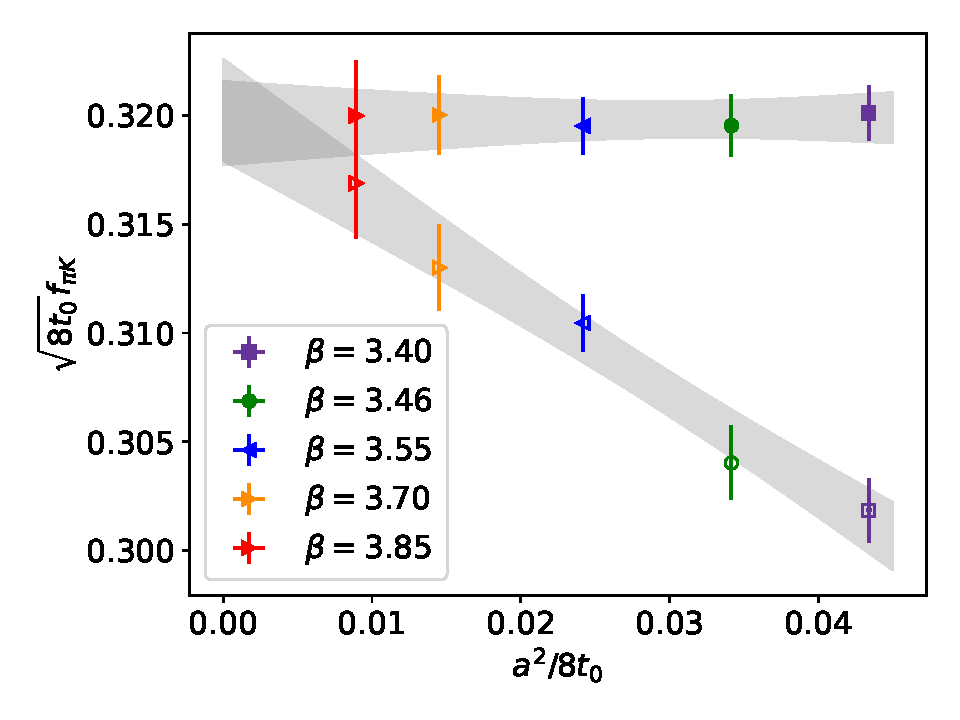
\includegraphics[width=1.\textwidth]{./cap5/figs/continuum_sym.pdf}
    \caption{Continuum limit of symmetric point ensembles for the Wilson unitary results (empty points) and for the mixed action results (filled points). In order to perform a universality check and verify that both regularizations share the same continuum limit, a common result at vanishing lattice spacing is not imposed. Cutoff effects are parameterized as pure $\mathcal{O}(a^2)$ artifacts independent for each regularization.}
    \label{ch_ss:fig:universality}
\end{figure}

\begin{figure}
    \centering
    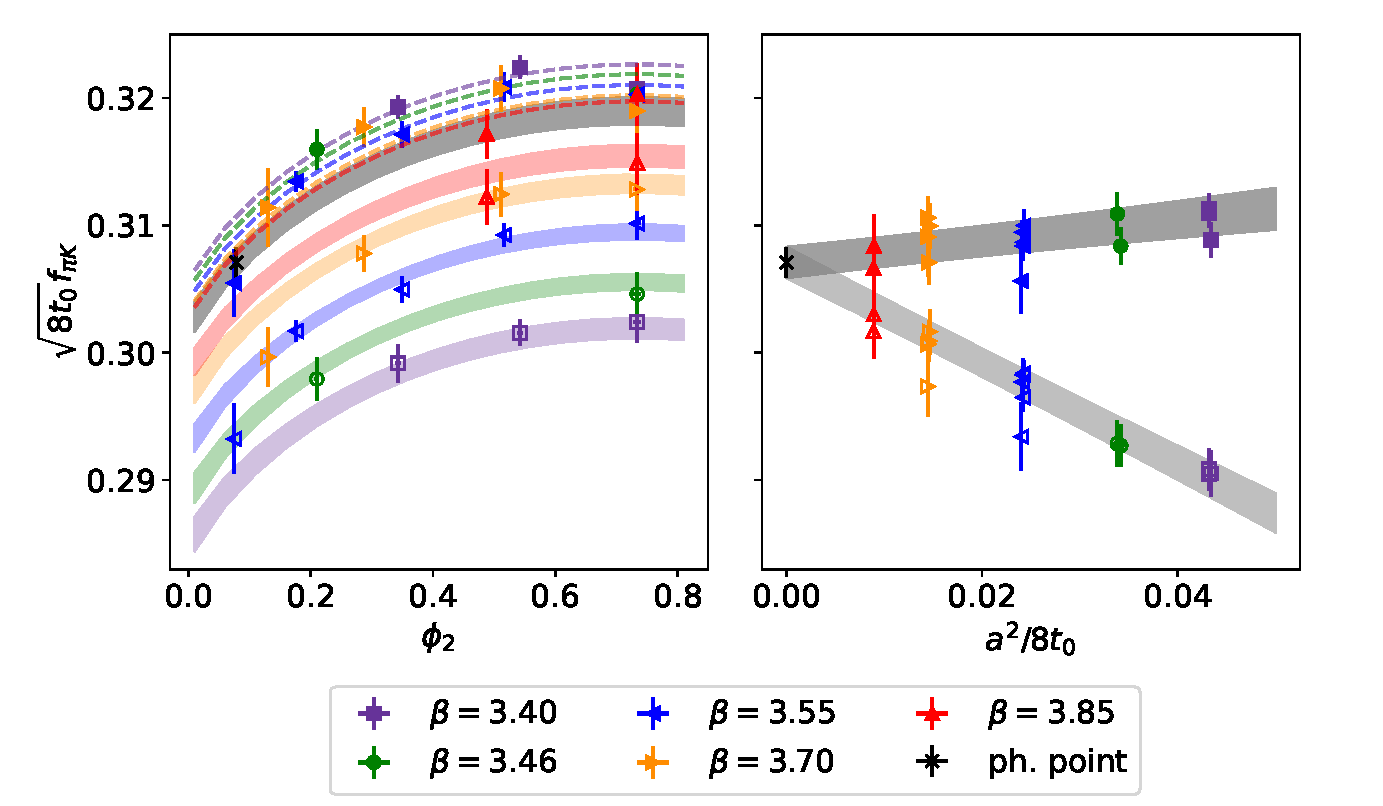
\includegraphics[width=1.\textwidth]{./cap5/figs/SU3_comb.pdf}
    \caption{\textit{Left}: Pion mass dependence of $\sqrt{8t_0}f_{\pi K}$ for the $SU(3)$ ChPT model with pure $\mathcal{O}(a^2)$ cutoff effects and no cut in data: $[SU(3)\chi PT][a^2][-]$. We show the result of the combined fit of both Wilson (empty) and mixed action (filled) results. The colored bands represent the pion mass dependence for each lattice spacing for the Wilson results, while the dashed lines represent the dependence for the mixed action results. In the latter case we only plot the central value of the corresponding bands for visualization purposes. \textit{Right}: the same model, with points projected to the physical pion mass $\phi_2^{\textrm{ph}}$ using the fit result for the continuum mass dependence $F(\phi_2)^{\textrm{cont}}$. In this plot we show the lattice spacing dependence of our ensembles. We show two physical point results: the rightmost in the plot corresponds to the result coming from the fit model itself, while the leftmost is the result obtained from the model average.}
    \label{ch_ss:fig:SU3a2}
\end{figure}

\begin{figure}
    \centering
    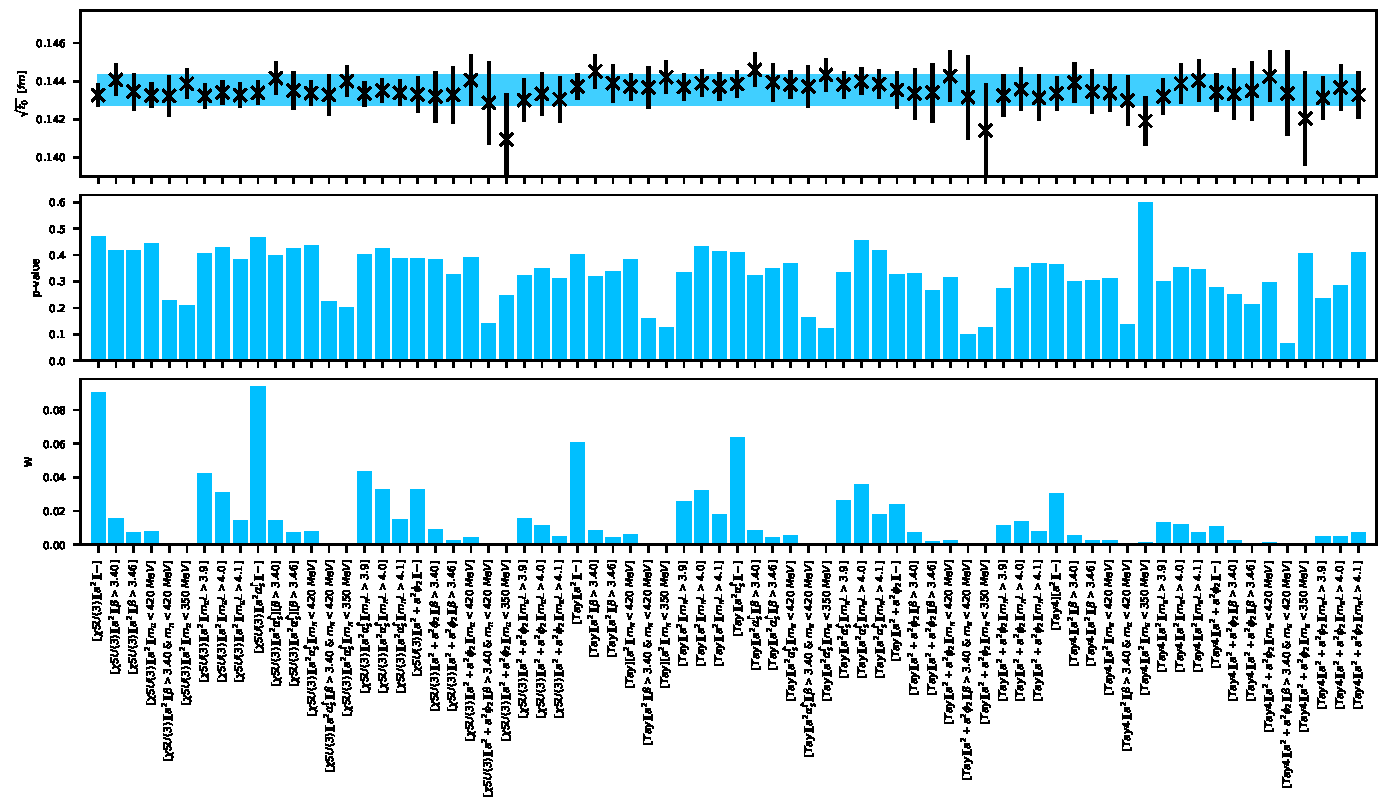
\includegraphics[width=1.\textwidth]{./cap5/figs/BMA_w.pdf}
    \caption{Model average results for the determination of $\sqrt{t_0}$ at the physical point using the Wilson results and $f_{\pi K}$ as physical input. In the leftmost figure we show the results coming from each fit model together with the final averaged result with the systematic uncertainty coming from the model variation added (blue band). In the middle plot we show the quality of fits as measured by the p-value~\citep{Bruno:2022mfy}. In the rightmost figure we show the assigned weight to each model according to eq.~(\ref{ch_ss:eq:W}). We provide a Table connecting each label to the corresponding fit models in Appendix~\ref{apex_model_av_t0}.}
    \label{ch_ss:fig:BMA_w}
\end{figure}

\begin{figure}
    \centering
    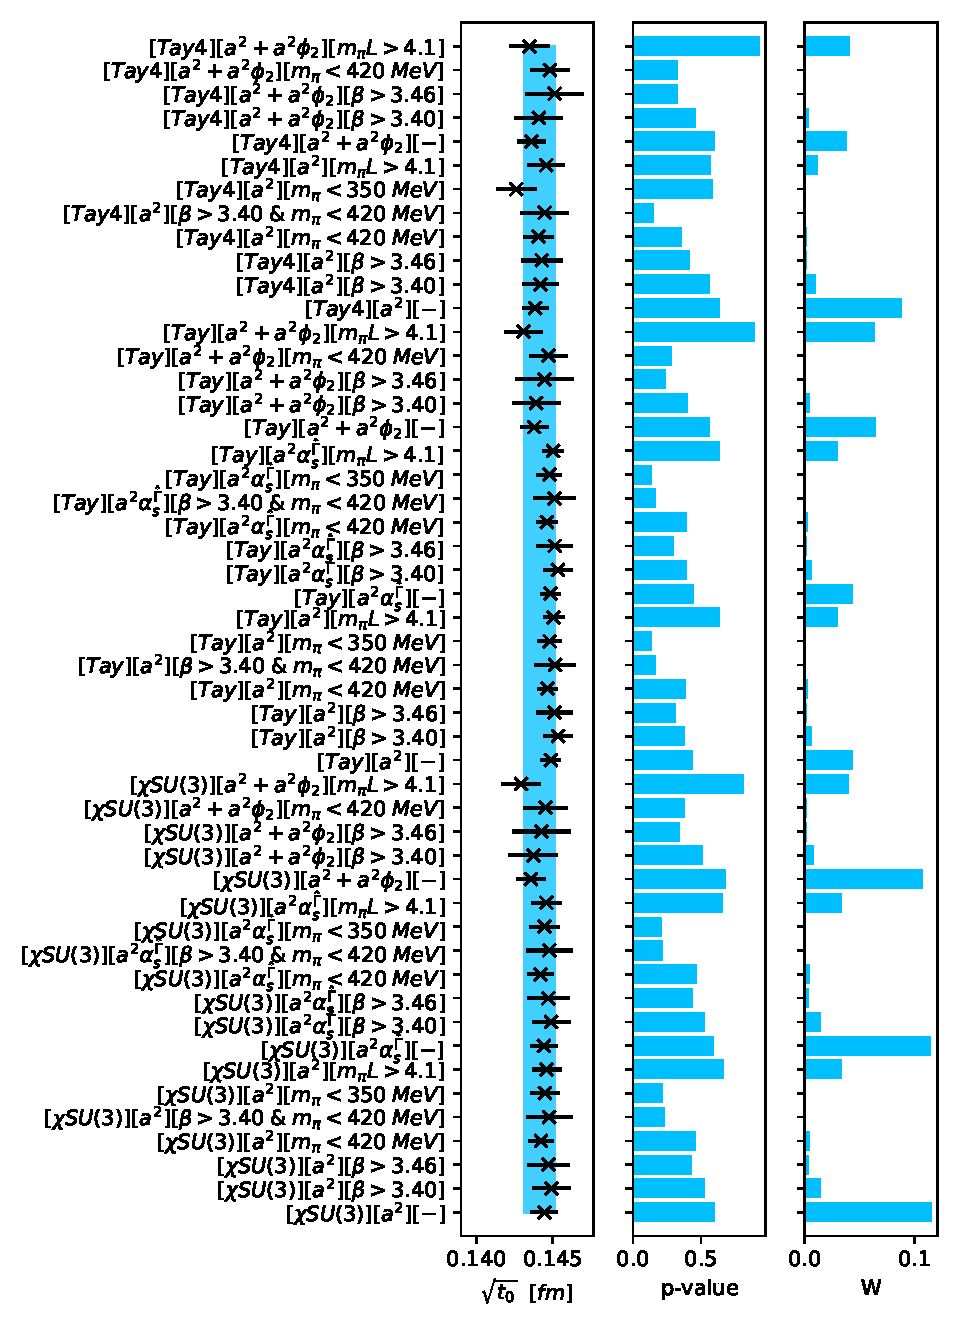
\includegraphics[width=1.\textwidth]{./cap5/figs/BMA_tm.pdf}
    \caption{Model average results for the determination of $\sqrt{t_0}$ at the physical point using the mixed action results and $f_{\pi K}$ as physical input. In the leftmost figure we show the results coming from each fit model together with the final averaged result with the systematic uncertainty coming from the model variation added (blue band). In the middle plot we show the quality of fits as measured by the p-value~\citep{Bruno:2022mfy}. In the rightmost figure we show the assigned weight to each model according to eq.~(\ref{ch_ss:eq:W}). We provide a Table connecting each label to the corresponding fit models in Appendix~\ref{apex_model_av_t0}.}
    \label{ch_ss:fig:BMA_tm}
\end{figure}

\begin{figure}
    \centering
    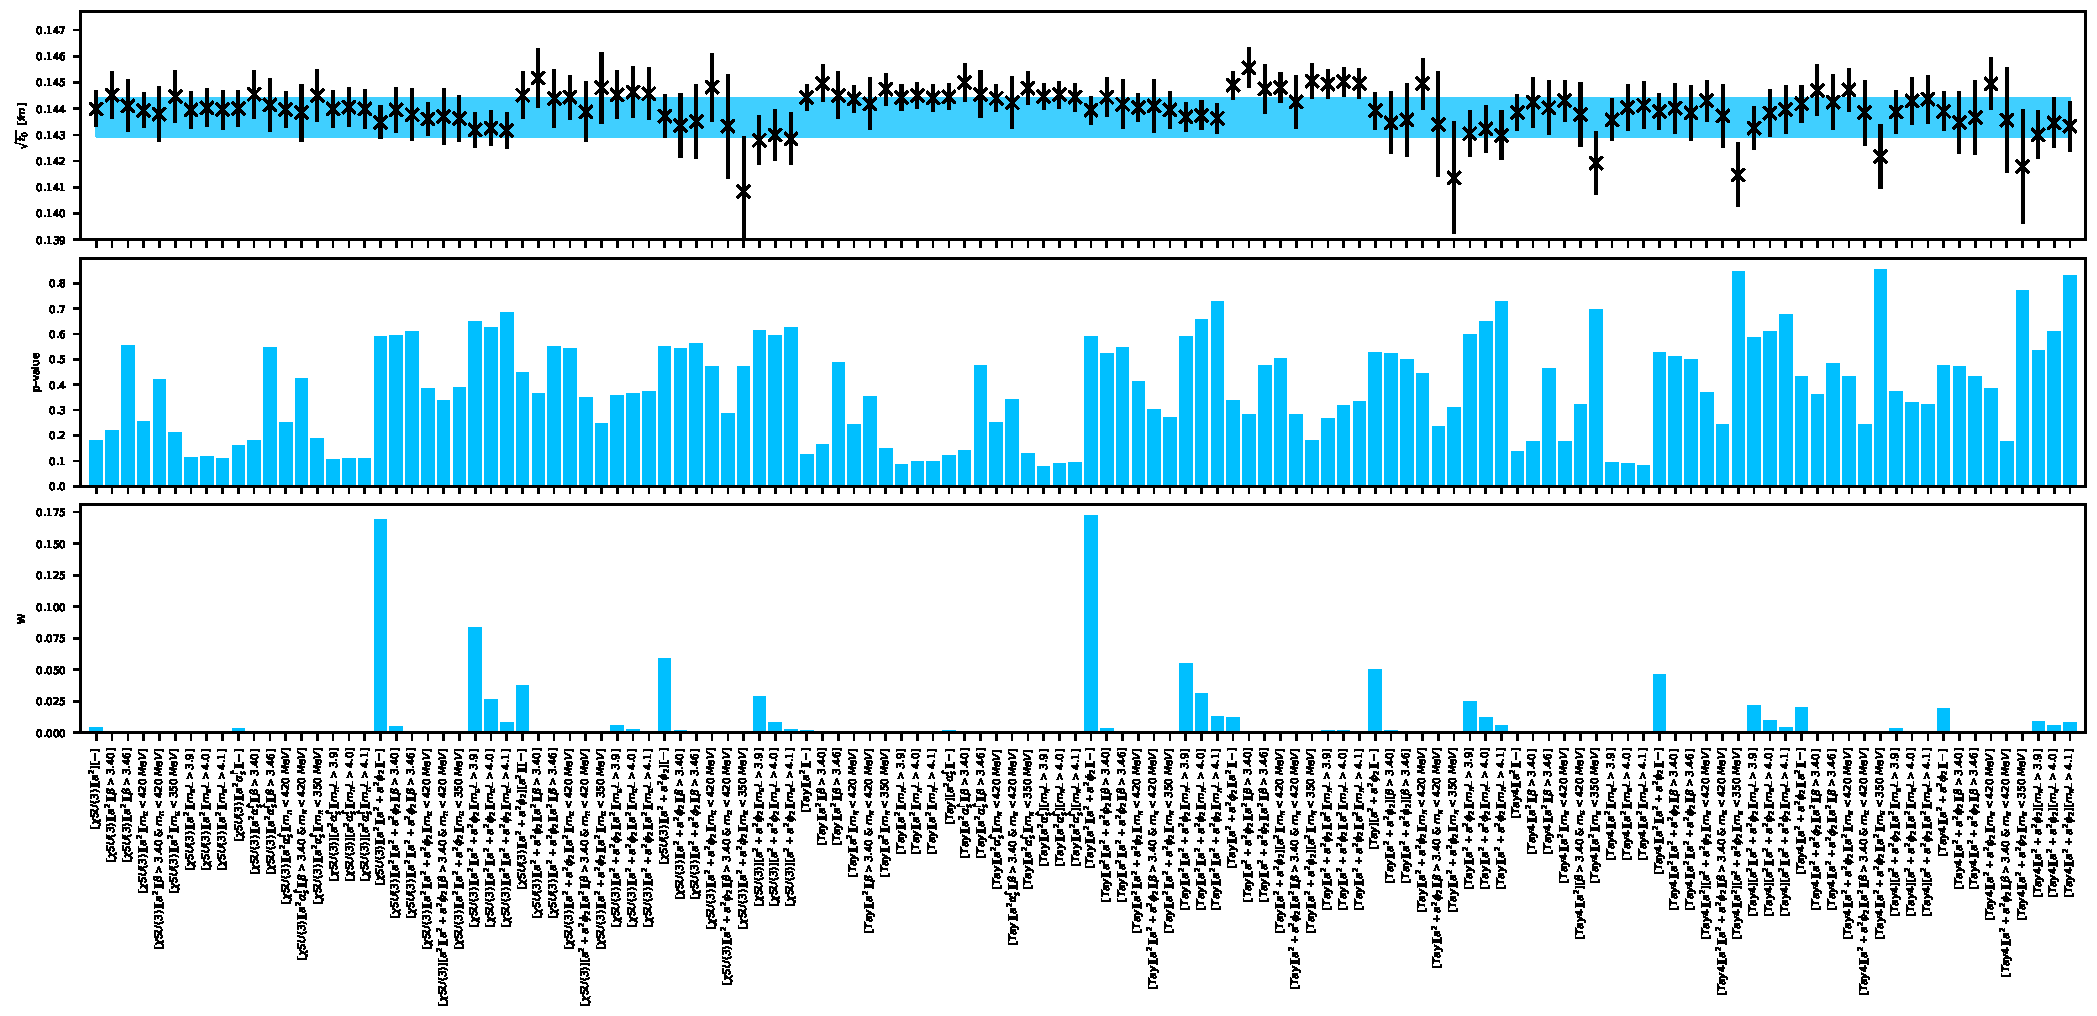
\includegraphics[width=1.\textwidth]{./cap5/figs/BMA_comb.pdf}
    \caption{Model average results for the determination of $\sqrt{t_0}$ at the physical point using the combined analysis of both Wilson and mixed action results and $f_{\pi K}$ as physical input. In the leftmost figure we show the results coming from each fit model together with the final averaged result with the systematic uncertainty coming from the model variation added (blue band). In the middle plot we show the quality of fits as measured by the p-value~\citep{Bruno:2022mfy}. In the rightmost figure we show the assigned weight to each model according to eq.~(\ref{ch_ss:eq:W}). We provide a Table connecting each label to the corresponding fit models in Appendix~\ref{apex_model_av_t0}.}
    \label{ch_ss:fig:BMA_comb}
\end{figure}

\begin{figure}
    \centering
    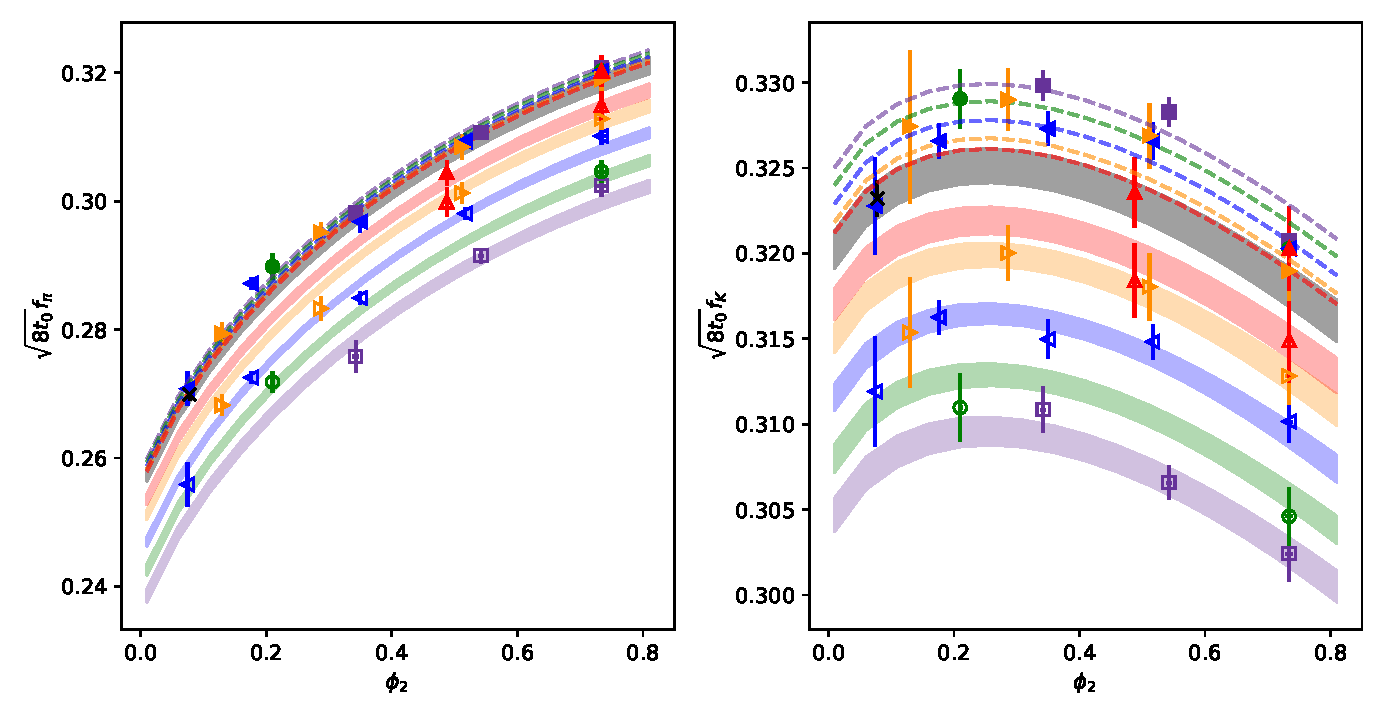
\includegraphics[width=1.\textwidth]{./cap5/figs/SU2_comb.pdf}
    \caption{\textit{Left}: Pion mass dependence of $\sqrt{8t_0}f_{\pi}$ for the $SU(2)$ ChPT model with pure $\mathcal{O}(a^2)$ cutoff effects and no cut in data: $[SU(2)\chi PT][a^2][-]$. We show the result of the combined fit of both Wilson (empty) and mixed action (filled) results. The colored bands represent the pion mass dependence for each lattice spacing for the Wilson results, while the dashed lines represent the dependence for the mixed action results. In the latter case we only plot the central value of the corresponding bands for visualization purposes. \textit{Right}: the same but for the dependence of $\sqrt{8t_0}f_{K}$. The color and symbol code is the same as in Fig.~\ref{ch_ss:fig:SU3a2}.}
    \label{ch_ss:fig:SU2_comb}
\end{figure}

\begin{figure}
    \centering
    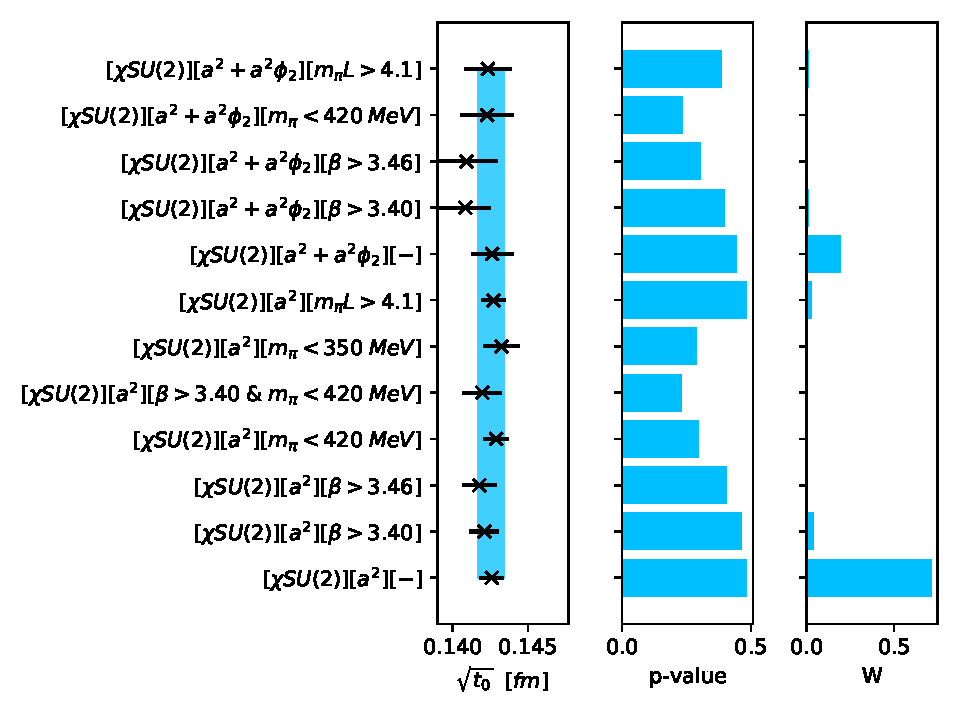
\includegraphics[width=1.\textwidth]{./cap5/figs/BMA_SU2_w.pdf}
    \caption{Model average results for the determination of $\sqrt{t_0}$ at the physical point using the Wilson results and $f_{\pi}$ as physical input. In the leftmost figure we show the results coming from each fit model together with the final averaged result with the systematic uncertainty coming from the model variation added (blue band). In the middle plot we show the quality of fits as measured by the p-value~\citep{Bruno:2022mfy}. In the rightmost figure we show the assigned weight to each model according to eq.~(\ref{ch_ss:eq:W}). We provide a Table connecting each label to the corresponding fit models in Appendix~\ref{apex_model_av_t0}.}
    \label{ch_ss:fig:BMA_w_SU2}
\end{figure}

\begin{figure}
    \centering
    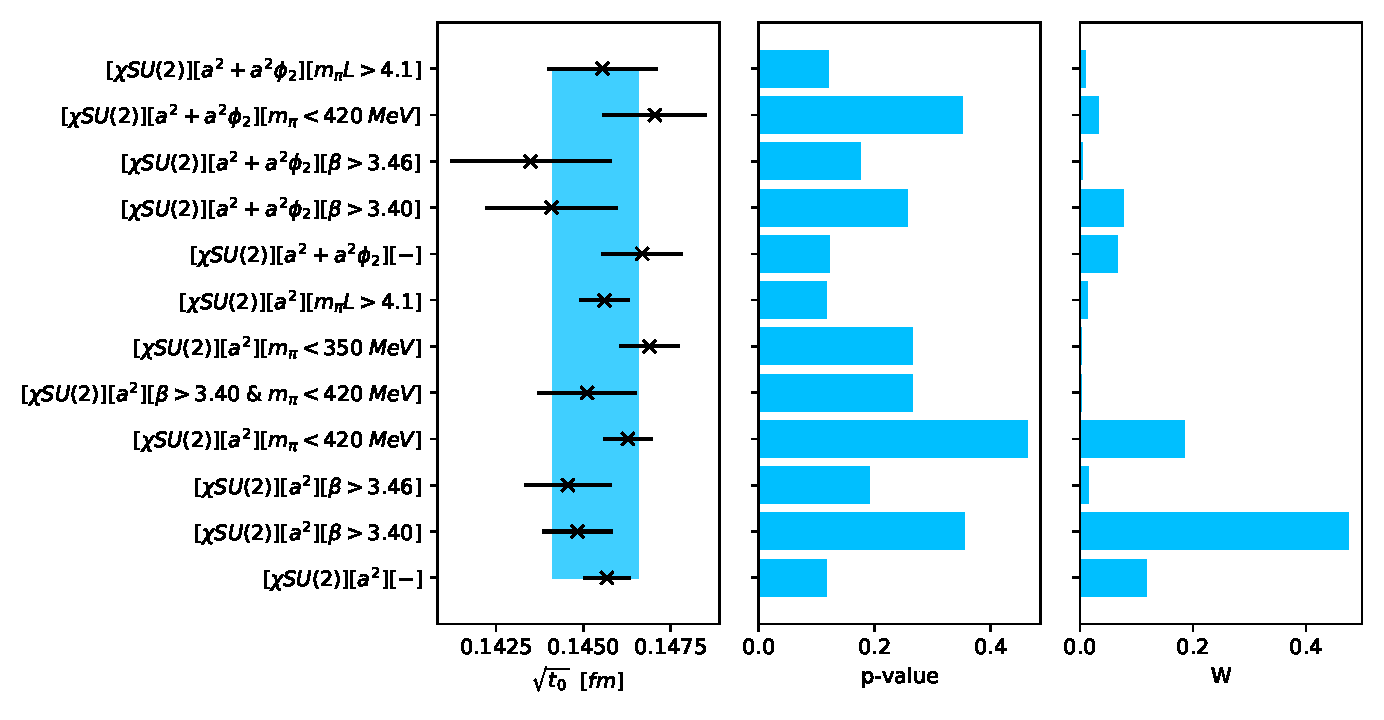
\includegraphics[width=1.\textwidth]{./cap5/figs/BMA_SU2_tm.pdf}
    \caption{Model average results for the determination of $\sqrt{t_0}$ at the physical point using the mixed action results and $f_{\pi}$ as physical input. In the leftmost figure we show the results coming from each fit model together with the final averaged result with the systematic uncertainty coming from the model variation added (blue band). In the middle plot we show the quality of fits as measured by the p-value~\citep{Bruno:2022mfy}. In the rightmost figure we show the assigned weight to each model according to eq.~(\ref{ch_ss:eq:W}). We provide a Table connecting each label to the corresponding fit models in Appendix~\ref{apex_model_av_t0}.}
    \label{ch_ss:fig:BMA_tm_SU2}
\end{figure}

\begin{figure}
    \centering
    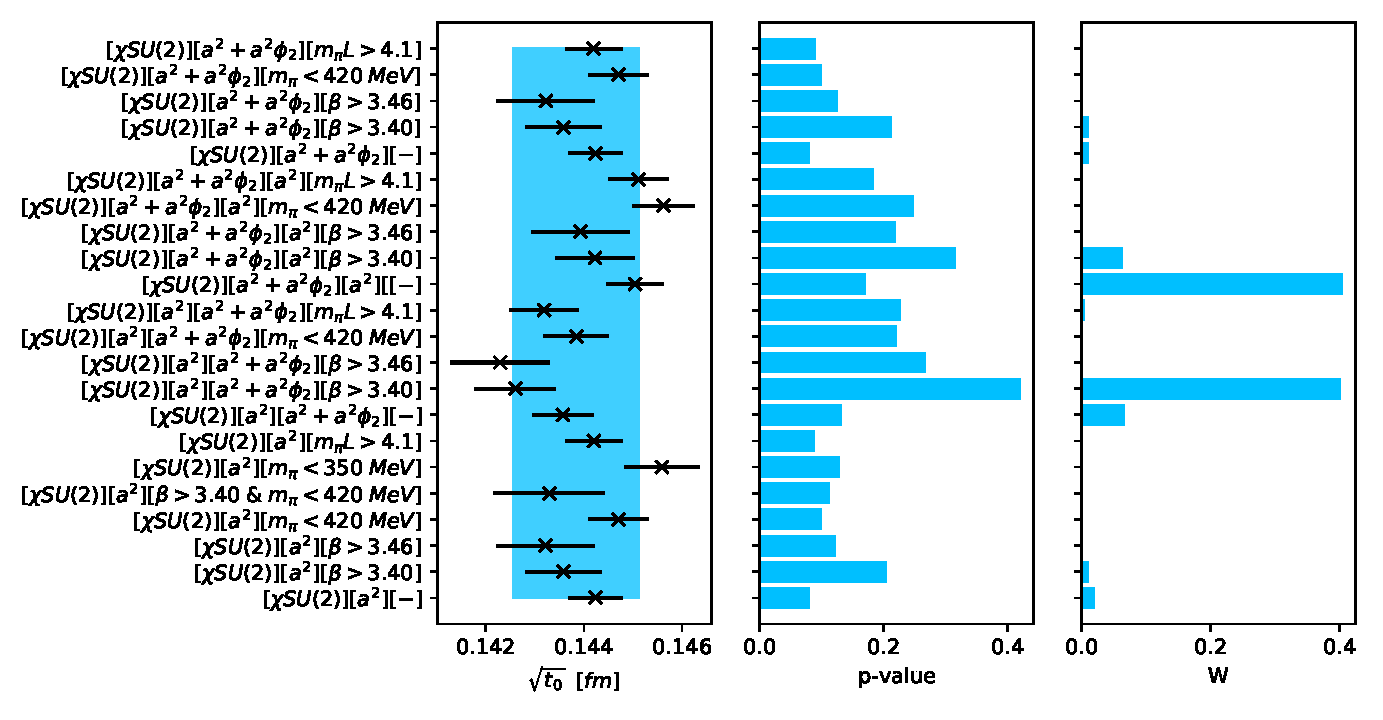
\includegraphics[width=1.\textwidth]{./cap5/figs/BMA_SU2_comb.pdf}
    \caption{Model average results for the determination of $\sqrt{t_0}$ at the physical point using the combined analysis of both Wilson and mixed action results and $f_{\pi}$ as physical input. In the leftmost figure we show the results coming from each fit model together with the final averaged result with the systematic uncertainty coming from the model variation added (blue band). In the middle plot we show the quality of fits as measured by the p-value~\citep{Bruno:2022mfy}. In the rightmost figure we show the assigned weight to each model according to eq.~(\ref{ch_ss:eq:W}). We provide a Table connecting each label to the corresponding fit models in Appendix~\ref{apex_model_av_t0}.}
    \label{ch_ss:fig:BMA_comb_SU2}
\end{figure}

\section{Results: the symmetric point}

The symmetric point is defined as the point in the quark mass plane such that
\begin{equation}
m_{ud}\equiv m_l=m_s.
\end{equation}
In terms of our usual quantities $\phi_2,\phi_4$ this means
\begin{equation}
\phi_2=\frac{2}{3}\phi_4,
\end{equation}
where $\phi_4$ again is given by its physical value after the iterative procedure to find $t_0^{\textrm{ph}}$ and after mass shifting (see Sec.~\ref{ch_ma:sec:chiral_traj}). In order to extract $t_0^{\textrm{sym}}=t_0(\phi_2^{\textrm{sym}},\phi_4^{\textrm{ph}})$, following~\citep{Strassberger:2023xnj} we build the ratio
\begin{equation}
\frac{\sqrt{t_0/a^2}}{\sqrt{t_0^{\textrm{sym}}/a^2}},
\end{equation}
where $\sqrt{t_0/a^2}$ is the measurement of the gradient flow scale in each ensemble and $\sqrt{t_0^{\textrm{sym}}/a^2}$ is said quantity for the symmetric point at the corresponding value of the inverse coupling $\beta$. We now fit this ratio to
\begin{equation}
\label{ch_ss:eq:fit_t0_sym}
F(\phi_2)=\sqrt{1+p(\phi_2-\phi_2^{\textrm{sym}})}.
\end{equation}
The result of this fit is shown in Fig.~\ref{ch_ss:fig:t0_sym}. Once the data is fitted, we extract $t_0^{\textrm{sym}}$ in physical units as
\begin{equation}
\sqrt{t_0^{\textrm{sym}}}=\frac{\sqrt{t_0^{\textrm{ph}}}}{F(\phi_2^{\textrm{ph}})}.
\end{equation}
For $t_0^{\textrm{ph}}$ and $\phi_2^{\textrm{ph}}$ we can use our determination for the Wilson, mixed action or combined data sets. The result for the scale at the symmetric point is, depending on this choice
\begin{align}
\label{ch_ss:eq:t0_sym}
\sqrt{t_0^{\textrm{sym}}}&=0.1433(8)_{\textrm{stat}}(3)_{\textrm{syst}}\;\textrm{fm, Wilson}, \\
\sqrt{t_0^{\textrm{sym}}}&=0.1438(8)_{\textrm{stat}}(6)_{\textrm{syst}}\;\textrm{fm, Mixed action}, \\
\sqrt{t_0^{\textrm{sym}}}&=0.1437(6)_{\textrm{stat}}(4)_{\textrm{syst}}\;\textrm{fm, Combined}.
\end{align}

\begin{figure}
    \centering
    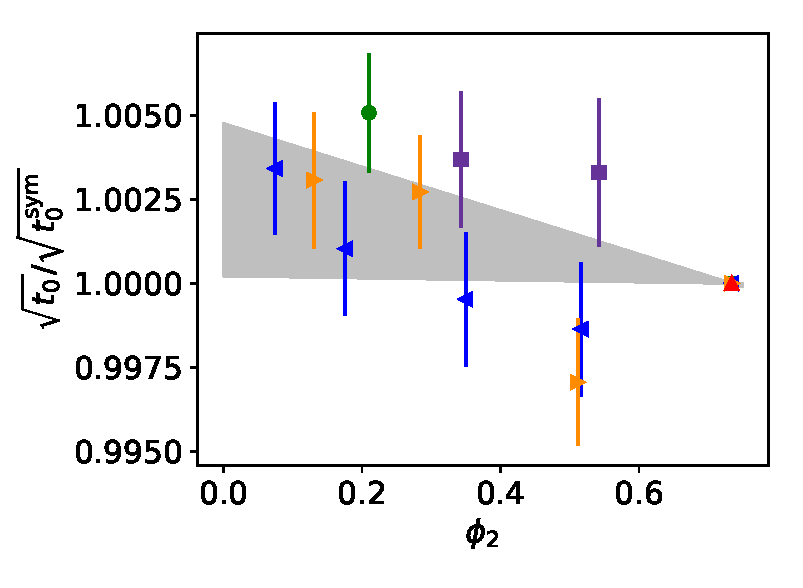
\includegraphics[width=.7\textwidth]{./cap5/figs/t0_sym.pdf}
    \caption{Fit to eq.~(\ref{ch_ss:eq:fit_t0_sym}) in order to extract $t_0$ at the symmetric point. The color and symbol code is the same as in Fig.~\ref{ch_ss:fig:SU3a2}.}
    \label{ch_ss:fig:t0_sym}
\end{figure}

\section{Results: lattice spacing}
\label{ch_ss:sec:t0_sym}

Just as in the previous section, we can use the fit to $\frac{\sqrt{t_0/a^2}}{\sqrt{t_0^{\textrm{sym}}/a^2}}$ to compute 
\begin{equation}
\left(\sqrt{\frac{t_0}{a^2}}\right)^{\textrm{ph}}=\sqrt{\frac{t_0^{\textrm{sym}}}{a^2}}F(\phi_2^{\textrm{ph}}).
\end{equation}
Then, the lattice spacing is extracted as
\begin{equation}
\label{ch_ss:eq:a}
a=\frac{\sqrt{t_0^{\textrm{ph}}}}{\left(\sqrt{\frac{t_0}{a^2}}\right)^{\textrm{ph}}}.
\end{equation}
Again, for $\phi_2^{\textrm{ph}}$ we can use either our determination of $t_0^{\textrm{ph}}$ for the Wilson, mixed action or combined data sets. Results for the lattice spacing are shown in Table~\ref{ch_ss:tab:a}.

\begin{longtable}{c c c c}
\label{ch_ss:tab:a}
$\beta$ & $a$ [fm] Wilson & $a$ [fm] mixed action & $a$ [fm] combined \\
\toprule
$3.40$ & $0.0844(5)_{\textrm{stat}}(2)_{\textrm{syst}}$ & $0.0848(5)_{\textrm{stat}}(4)_{\textrm{syst}}$ & $0.0847(4)_{\textrm{stat}}(2)_{\textrm{syst}}$ \\
$3.46$ & $0.0749(4)_{\textrm{stat}}(2)_{\textrm{syst}}$ & $0.0752(4)_{\textrm{stat}}(3)_{\textrm{syst}}$ & $0.0751(3)_{\textrm{stat}}(2)_{\textrm{syst}}$ \\
$3.55$ & $0.0630(3)_{\textrm{stat}}(2)_{\textrm{syst}}$ & $0.0632(3)_{\textrm{stat}}(3)_{\textrm{syst}}$ & $0.0632(3)_{\textrm{stat}}(2)_{\textrm{syst}}$ \\
$3.70$ & $0.0489(3)_{\textrm{stat}}(1)_{\textrm{syst}}$ & $0.0490(3)_{\textrm{stat}}(2)_{\textrm{syst}}$ & $0.0490(2)_{\textrm{stat}}(1)_{\textrm{syst}}$ \\
$3.85$ & $0.0383(2)_{\textrm{stat}}(1)_{\textrm{syst}}$ & $0.0385(2)_{\textrm{stat}}(2)_{\textrm{syst}}$ & $0.0384(2)_{\textrm{stat}}(1)_{\textrm{syst}}$ \\
\bottomrule
\caption{Values of the lattice spacing $a$ in physical units extracted from the determination of the gradient flow scale $t_0$ with the Wilson, mixed action and combined analysis. The lattice spacing is extracted from measures of both $t_0$ at the physical and symmetric points using eq.~(\ref{ch_ss:eq:a}).}
\end{longtable}

\section{Results: $t_0^*$}

Another point in the $(\phi_2,\phi_4)$ plane of interest is the reference point in~\citep{Bruno:2016plf}
\begin{gather}
\phi_4=1.11, \quad \phi_2=\frac{2}{3}\phi_4\equiv\phi_2^{\textrm{sym}}.
\end{gather}
The scale $t_0$ evaluated at this point is
\begin{equation}
t_0^*=t_0\left(\phi_2^{\textrm{sym}},\;\phi_4=1.11\right),
\end{equation}
and its ratio to $\sqrt{t_0^{\textrm{ph}}}$ plays a crucial role in the computation of the strong coupling in~\citep{DallaBrida:2022eua}. To compute $t_0^{*}$, we need to repeat the analysis above, this time mass shifting our ensembles to the value $\phi_4=1.11$ without errors and compute the gradient flow scale at the symmetric point as explained in the Sec.~\ref{ch_ss:sec:t0_sym}.

The values we find for $\sqrt{t_0^*}$ in physical units for the Wilson, mixed action and combined cases are
\begin{align}
\label{ch_ss:eq:t0*}
\sqrt{t_0^*}&=0.1436(7)_{\textrm{stat}}(4)_{\textrm{syst}}\;\textrm{fm, Wilson}, \\
\sqrt{t_0^*}&=0.1441(7)_{\textrm{stat}}(5)_{\textrm{syst}}\;\textrm{fm, Mixed action}, \\
\sqrt{t_0^*}&=0.1438(6)_{\textrm{stat}}(3)_{\textrm{syst}}\;\textrm{fm, Combined}.
\end{align}

%%%%%%%%%%%%%%%%%%%%%%%%%%%%%%%%%%%%%%%%%%%%%%%%%%%%%%%%%%%
%%%%%%%%%%%%%%%%%%%%%%%%%%%%%%%%%%%%%%%%%%%%%%%%%%%%%%%%%%%
%%%%%%%%%%%%%%%%%%%%%%%%%%%%%%%%%%%%%%%%%%%%%%%%%%%%%%%%%%%
%%%%%%%%%%%%%%%%%%%%%%%%%%%%%%%%%%%%%%%%%%%%%%%%%%%%%%%%%%%
